\documentclass{beamer}
\usetheme{CambridgeUS}

\setbeamertemplate{caption}[numbered]{}

\usepackage{amsmath}
\usepackage{amssymb}
\usepackage{gensymb}
\usepackage{graphicx}
\usepackage{txfonts}

\def\inputGnumericTable{}

\usepackage[latin1]{inputenc}                                 
\usepackage{color}                                            
\usepackage{array}                                            
\usepackage{longtable}                                        
\usepackage{calc}                                             
\usepackage{multirow}                                         
\usepackage{hhline}                                           
\usepackage{ifthen}
\usepackage{caption} 
\captionsetup[table]{skip=3pt}

\providecommand{\pr}[1]{\ensuremath{\Pr\left(#1\right)}}
\providecommand{\brak}[1]{\ensuremath{\left(#1\right)}}
\providecommand{\cbrak}[1]{\ensuremath{\left\{#1\right\}}}

\renewcommand{\thefigure}{\arabic{table}}
\renewcommand{\thetable}{\arabic{table}}                                     
                               
\title{AI1110 \\ Assignment 13}
\author{Ankit Saha \\ AI21BTECH11004}
\date{26 May 2022}


\begin{document}
	% The title page
	\begin{frame}
		\titlepage
	\end{frame}
	
	% The table of contents
	\begin{frame}{Outline}
    		\tableofcontents
	\end{frame}
	
	% The question
	\section{Question}
	\begin{frame}{Papoulis Exercise 5-51}
	A box contains $N$ identical items of which $M < N$ are defective ones. A sample of size $n$ is taken from the box, and let $X$ represent the number of defective items in the sample.  
	\begin{enumerate}
	\item Find the distribution function of $X$ if the $n$ samples are drawn with replacement.
	\item If the $n$ samples are drawn without replacement, then show that 
	\begin{align}
		\pr{X=k} = \frac{\binom{M}{k} \binom{N-M}{n-k}}{\binom{N}{n}} \quad \max(0, n+M-N) \le k \le \min(M,n)
	\end{align}
	Find the mean and variance of $X$. This distribution is known as the hypergeometric distribution.
	\end{enumerate}
	\end{frame}
	
	\begin{frame}
		\begin{enumerate}
		\setcounter{enumi}{2}
		\item In the previous equation, let $N \to \infty, M \to \infty$ such that $\frac{M}{N} \to p, 0<p<1$. Then show that the hypergeometric random variable can be approximated by a binomial random variable with parameters $n$ and $p$ provided $n \ll N$
		\end{enumerate}
	\end{frame}
	
	% The solution
	\section{First Part}
	\begin{frame}{First Part}
		Let there be $k$ defective items among the $n$ chosen samples. Since we are drawing with replacement, the distribution will be a binomial distribution with parameters $n$ and $p = \frac{M}{N}$ where $p$ is the probability that a randomly chosen sample is defective.
		\begin{align}
			f_X(k) &= \binom{n}{k} p^k (1-p)^{n-k}, ~k \in \cbrak{0,1,\ldots,n} \\
			&= \binom{n}{k} \brak{\frac{M}{N}}^k \brak{\frac{N-M}{N}}^{n-k}, ~k \in \cbrak{0,1,\ldots,n} \\
			&= \binom{n}{k} \frac{M^k (N-M)^{n-k}}{N^n}, ~k \in \cbrak{0,1,\ldots,n}
		\end{align}
	\end{frame}
	
	\section{Second Part}
	\begin{frame}{Second Part}
	Now we are drawing without replacement. $n$ samples can be chosen from $N$ items in $\binom{N}{n}$ ways. Out of these, $k$ defective samples can be chosen from a total of $M$ defective items in $\binom{M}{k}$ ways and the remaining $n-k$ samples can be chosen from the $N-M$ non-defective items in $\binom{N-M}{n-k}$ ways. Thus, the total number of ways of choosing $k$ defective and $n-k$ non-defective items is 
	\begin{align}
		\binom{M}{k} \binom{N-M}{n-k}
	\end{align}
	Therefore, the probability is given by
	\begin{align}
		\pr{X=k} = \frac{\binom{M}{k} \binom{N-M}{n-k}}{\binom{N}{n}}
	\end{align}
	\end{frame}
	
	\begin{frame}
	The constraints on $k$ can be obtained as follows:
	\begin{align}
		&k \ge 0, n-k \le N-M \\
		&\implies k \ge \max(0, n+M-N) \\
		&k \le M, n - k \ge 0 \\
		&\implies k \le \min(M,n) \\
		&\therefore \max(0, n+M-N) \le k \le \min(M,n)
	\end{align}	 
	\end{frame}
	
	\begin{frame}{Mean}
	The mean of $X$ is given by
	\begin{align}
		E[X] &= \sum_k k \pr{X=k} \\
		&= \sum_k \frac{k \binom{M}{k} \binom{N-M}{n-k}}{\binom{N}{n}} \\
		k \binom{M}{k} = k \frac{M!}{k!(M-k)!} &= M \frac{(M-1)!}{(k-1)!(M-k)!} = M \binom{M-1}{k-1} \\
		\binom{N}{n} = \frac{N!}{n!(N-n)!} &= \frac{N}{n} \frac{(N-1)!}{(n-1)!(N-n)!} = \frac{N}{n} \binom{N-1}{n-1} \\
		\implies E[X] &= \sum_k \frac{M \binom{M-1}{k-1} \binom{N-M}{n-k}}{\frac{N}{n} \binom{N-1}{n-1}} 
	\end{align}
	\end{frame}
	
	\begin{frame}
	\begin{align}
		E[X] = \frac{Mn}{N} \frac{\sum_k \binom{M-1}{k-1} \binom{N-M}{n-k}}{\binom{N-1}{n-1}}
	\end{align}
	By Vandermonde's identity,
	\begin{align}
		\sum_i \binom{a}{i}\binom{b}{r-i} &= \binom{a+b}{r}
	\end{align}
	Combinatorially, this can be shown by counting the number of ways to select $r$ fruits from a basket consisting of $a$ apples and $b$ oranges. This is equal to the sum over all possible values of $i$, of the number of ways to select $i$ apples and $r-i$ oranges.
	\end{frame}
	
	\begin{frame}
	\begin{align}
		\implies \sum_k \binom{M-1}{k-1} \binom{N-M}{n-k} &= \sum_k \binom{M-1}{k-1} \binom{N-M}{(n-1)-(k-1)} \\
		&= \binom{N-1}{n-1} \\
		\implies \frac{\sum_k \binom{M-1}{k-1} \binom{N-M}{n-k}}{\binom{N-1}{n-1}} &= 1
	\end{align}
	\begin{block}{}
	Therefore,
		\begin{align}
			E[X] = \frac{Mn}{N}
		\end{align}
	\end{block}
	\end{frame}
	
	\begin{frame}{Variance}
	The variance of $X$ is given by
	\begin{align}
		\mathrm{Var}(X) &= E[X^2] - \brak{E[X]}^2 \\
		E[X^2] &= \sum_k k^2 \pr{X=k} \\
		&= \sum_k \frac{k \cdot k \binom{M}{k} \binom{N-M}{n-k}}{\binom{N}{n}} \\
		&= \sum_k \frac{k \cdot M \binom{M-1}{k-1} \binom{N-M}{n-k}}{\binom{N}{n}} \\
		&= M \sum_k \frac{(k-1+1) \binom{M-1}{k-1} \binom{N-M}{n-k}}{\binom{N}{n}} \\
	\end{align}
	\end{frame}
	
	\begin{frame}
	\begin{align}
		E[X^2] &= M \sum_k \frac{(k-1) \binom{M-1}{k-1} \binom{N-M}{n-k}}{\frac{N(N-1)}{n(n-1)}\binom{N-2}{n-2}} + M \sum_k \frac{\binom{M-1}{k-1} \binom{N-M}{n-k}}{\frac{N}{n} \binom{N-1}{n-1}} \\ 
		&= \frac{Mn(n-1)}{N(N-1)} \sum_k \frac{(M-1) \binom{M-2}{k-2} \binom{N-M}{n-k}}{\binom{N-2}{n-2}} + \frac{Mn}{N} \\
		&= \frac{M(M-1)n(n-1)}{N(N-1)} + \frac{Mn}{N}
	\end{align}
	following a similar computation as that done for the mean
	\begin{align}
		\mathrm{Var}(X) &= E[X^2] - \brak{E[X]}^2 \\
		&= \frac{M(M-1)n(n-1)}{N(N-1)} + \frac{Mn}{N} - \brak{\frac{Mn}{N}}^2
	\end{align}
	\end{frame}
		
	\begin{frame}
	\begin{align}
		\mathrm{Var}(X) &= \frac{Mn}{N} \brak{\frac{(M-1)(n-1)}{N-1} + 1 - \frac{Mn}{N}} \\
		&= \frac{Mn}{N} \frac{N(M-1)(n-1) + N(N-1) - Mn(N-1)}{N(N-1)} \\
		&= \frac{Mn}{N^2(N-1)} \brak{NMn + N - NM - Nn + N^2 - N - NMn + Mn} \\
		&= \frac{Mn}{N^2(N-1)} (N(N-M) - n(N-M))
	\end{align}
	\begin{block}{}
	Therefore,
		\begin{align}
			\mathrm{Var}(X) = \frac{Mn(N-n)(N-M)}{N^2(N-1)}
		\end{align}
	\end{block}
	\end{frame}
	
	\begin{frame}{Plot of the distribution for $N=100, M=25, n=10$}
		\centering
		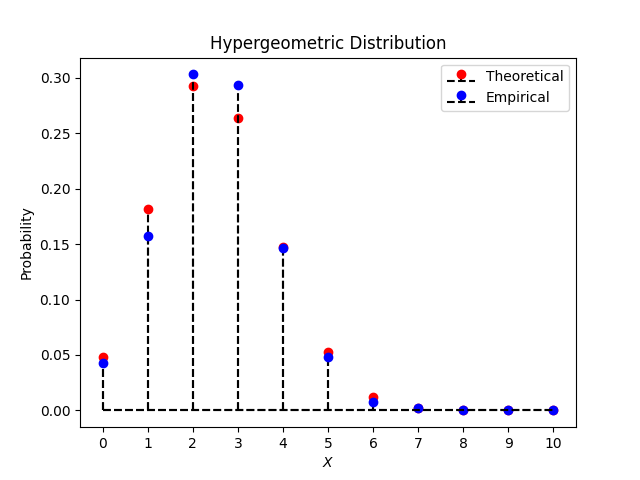
\includegraphics[height=0.8\paperheight]{figs/fig-1.png}
	\end{frame}
	
	\section{Third Part}
	\begin{frame}{Third Part}
	\begin{align}
		&\pr{X=k} \\
		&= \frac{\binom{M}{k} \binom{N-M}{n-k}}{\binom{N}{n}} \\
		&= \frac{M!}{k!(M-k)!} \frac{(N-M)!}{(n-k)!(N-M-n+k)!} \frac{n!(N-n)!}{N!} \\
		&= \frac{n!}{k!(n-k)!} \frac{M\cdots(M-k+1)}{N\cdots(N-k+1)} \frac{(N-M)\cdots(N-M-n+k+1)}{(N-k)\cdots(N-n+1)} \\
		&= \binom{n}{k} \frac{M^k \brak{1-\frac1M} \cdots \brak{1-\frac{k-1}{M}}}{N^k \brak{1-\frac1N} \cdots \brak{1-\frac{k-1}{N}}} \frac{(N-M)^{n-k} \brak{1-\frac{1}{N-M}} \cdots \brak{1-\frac{n-k-1}{N-M}}}{(N-k)^{n-k} \brak{1-\frac{1}{N-k}} \cdots \brak{1-\frac{n-k-1}{N-k}}}
	\end{align}
	\end{frame}
	
	\begin{frame}
	Now, $N \to \infty, M \to \infty$ such that $\frac{M}{N} \to p, 0<p<1$
	\begin{align}
		&\implies N-M \simeq N(1-p) \to \infty \\
		&\text{and } k \le n \ll N \implies N-k \simeq N \to \infty
	\end{align}
	Thus,
	\begin{align}
		\pr{X=k} &\simeq \binom{n}{k} \frac{M^k}{N^k} \frac{(N-M)^{n-k}}{N^{n-k}} \\
		&= \binom{n}{k} p^k (1-p)^{n-k}
	\end{align}
	where $p = \frac{M}{N}$
	
	Therefore, the hypergeometric random variable can be approximated by a binomial random variable with parameters $n$ and $k$. $\qed$
	\end{frame}
	
	\begin{frame}{Plot as $N, M \to \infty, \frac{M}{N} \to p, 0 < p < 1, n \ll N$}
		\centering
		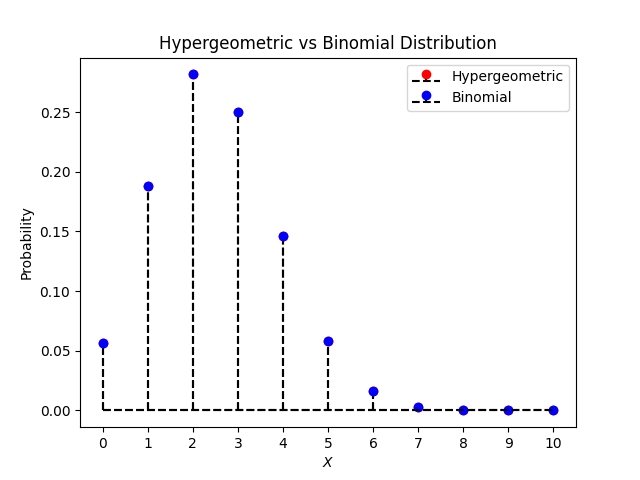
\includegraphics[height=0.8\paperheight]{figs/fig-2.png}
	\end{frame}
	
\end{document}